\documentclass[10pt]{article}

%---------------------------------------------------------------------------------------------------------------------------------------------
% Including Packages
\usepackage{nips13submit_e,times}
\usepackage{color}
\usepackage{algorithm2e}
\usepackage{ mathrsfs }
\usepackage{ dsfont }
\usepackage{lmodern}
\usepackage{array}
\usepackage{bbm}
\usepackage{amsmath}
\usepackage{amssymb}
\usepackage[mathscr]{eucal}
\usepackage{graphicx}
\usepackage{mathrsfs}
\usepackage{psfrag}
\usepackage{color}
\usepackage{here}
\usepackage{amsthm}
\usepackage[margin=1in]{geometry}
%\usepackage[T1]{fontenc}
%\usepackage[charter]{mathdesign}
%\usepackage{eulervm}
\usepackage{enumitem}
\usepackage{xcolor}
\usepackage{caption}
\usepackage{subcaption}


\newtheorem{theorem}{Theorem}
\newtheorem{corollary}{Corollary}
\newtheorem{lemma}[theorem]{Lemma}
%---------------------------------------------------------------------------------------------------------------------------------------------
% Setting up macro shortcuts
\newcommand{\Exp}{\mathds{E}}
\newcommand{\Expk}{\mathds{E}_{k}}
\newcommand{\Prob}{\mathds{P}}
\newcommand{\Ind}{\mathds{1}}
\newcommand{\states}{\mathcal{S}}
\newcommand{\actions}{\mathcal{A}}
\newcommand{\confidence}{\mathcal{M}_k}
\newcommand{\vect}[1]{\boldsymbol{#1}}
\newcommand{\history}{\sigma ({H}_{t_k}) }
\newcommand{\opt}{M^*}
\newcommand{\sampled}{{M_k}}
\newcommand{\Pstar}{P^{*}(\cdot \mid s_t, a_t)} 
\newcommand{\Pk}{P_{k}(\cdot \mid s_t, a_t)}
\newcommand{\Pdiff}{(P_{k}-P^{*})(\cdot \mid s_t, a_t)}
\newcommand{\Rdiff}{(r_k-r^{*})(s_t, a_t)}

\newcommand{\optPol}{\mu^{*}}
\newcommand{\sampledPol}{\mu_{k}}
\newcommand{\bellmanSampled}{\mathcal{T}_{\mu_{k}(\cdot,i)}^{k}}
\newcommand{\bellmanTrue}{\mathcal{T}_{\mu_{k}(\cdot,i)}^{*}}
\newcommand{\bellmanSampledA}{\mathcal{T}_{\mu_{k}(\cdot,1)}^{k}}
\newcommand{\bellmanTrueA}{\mathcal{T}_{\mu_{k}(\cdot,1)}^{*}}
\newcommand{\vSampled}{V_{\mu_k, 1}^{k}}
\newcommand{\vSampledi}{V_{\mu_k, i}^{k}}
\newcommand{\vTrue}{V_{\tau, \mu_k}^{*}}

\newcommand{\thetaConf}{{\Theta}_k}
\newcommand{\ignorance}{ \| \vect{v}_{\opt,\sampledPol} ( P_{\sampled,\sampledPol} - P_{\opt,\sampledPol} ) \|_1}
\newcommand{\ignorancePhi}{ \| \vect{v}_{\opt,\mu_\phi} ( P_{\phi,\mu_\phi} - P_{\opt,\mu_\phi} ) \|_1}
\newcommand{\errorP}{ \| ( P_{\sampled,\sampledPol}(\dot | s_t,\sampledPol(s_t)) - P_{\opt,\sampledPol}(\dot | s_t,\sampledPol(s_t)) ) \|_1}
\newcommand{\samplespan}{\| \vect{\lambda_{\sampled,\sampledPol}} \|_{\infty}}


%---------------------------------------------------------------------------------------------------------------------------------------------

\title{(More) Efficient Reinforcement Learning via \\ Posterior Sampling}
\author{Ian Osband, Daniel Russo, Benjamin Van Roy}

%This is the author formatting given in the NIPS template. 
\author{
Ian Osband \\
Department of Management Science and Engineering\\
Stanford University \\
\And
Dan Russo \\
Department of Management Science and Engineering \\
Stanford Universit \\
\AND
Benjamin Van Roy \\
Departments of Management Science and Engineering and Electrical Engineering \\
Stanford University \\
}

% The \author macro works with any number of authors. There are two commands
% used to separate the names and addresses of multiple authors: \And and \AND.
%
% Using \And between authors leaves it to \LaTeX{} to determine where to break
% the lines. Using \AND forces a linebreak at that point. So, if \LaTeX{}
% puts 3 of 4 authors names on the first line, and the last on the second
% line, try using \AND instead of \And before the third author name.

\newcommand{\fix}{\marginpar{FIX}}
\newcommand{\new}{\marginpar{NEW}}

%\nipsfinalcopy % Uncomment for camera-ready version


\begin{document}
\maketitle

\begin{abstract}

Most provably-efficient learning algorithms introduce optimism about poorly-understood states and actions to encourage exploration. We study an alternative approach for efficient exploration, \emph{posterior sampling for reinforcement learning} (PSRL). This algorithm proceeds in repeated episodes of known duration. At the start of each episode, PSRL updates a prior distribution over Markov decision processes and takes one sample from this posterior. PSRL then follows the policy that is optimal for this \emph{sample} during the episode. The algorithm is conceptually simple, computationally efficient and allows an agent to encode prior knowledge in a natural way. We establish an $\tilde{O}(\tau S \sqrt{AT} )$ bound on the expected regret, where $T$ is time, $\tau$ is the episode length and $S$ and $A$ are the cardinalities of the state and action spaces. This bound is one of the first for an algorithm not based on optimism, and close to the state of the art for any reinforcement learning algorithm. We show through simulation that PSRL significantly outperforms existing algorithms with similar regret bounds.


\end{abstract}


%We propose PSRL: a computationally efficient reinforcement learning algorithm based upon posterior sampling. The algorithm proceeds in episodes of known duration. At the beginning of each, a posterior distribution over Markov decision processes is computed, an instance is sampled from this distribution, and an optimal reward for this \emph{sample} is computed for use over this episode. We establish an $\tilde{O}(\tau S \sqrt{AT} )$ bound on the expected regret, where $T$ is time, $S$ and $A$ are the cardinalities of the state and action spaces, and $\tau$ is the episode length. In doing this, we develop some of the first regret bounds for a reinforcement learning algorithm not based upon optimism. We show that these bounds hold in expectation irrespective of prior, and with high probability unless the prior misspecification is exponentially large. This algorithm is computationally efficient, since for each episode it only requires solving for an optimal policy of a single MDP; it allows an agent to encode prior knowledge in a natural way, which is invaluable for practical applications; and PSRL outperforms existing algorithms with similar regret bounds by large margins in simulation.


\section{Introduction}
We consider the classical reinforcement learning problem of an agent interacting with its environment while trying to maximize total reward accumulated over time \cite{burnetas1997optimal, kumar1986stochastic}. The agent's environment is 
modeled as a Markov decision process (MDP), but the agent is uncertain about the true dynamics of the MDP. As the agent interacts with its environment, it observes the outcomes that result from previous states and actions, and learns about the system dynamics. 
This leads to a fundamental tradeoff: by exploring poorly-understood states and actions the agent can learn to improve future performance, but it may attain better short-run performance by exploiting its existing knowledge.

Na\"ive optimization using point estimates for unknown variables overstates an agent's knowledge, which can lead to premature and suboptimal exploitation. To offset this, the majority of provably efficient learning algorithms use a principle known as \emph{optimism in the face of uncertainty} \cite{lai1985asymptotically} to encourage exploration. In such an algorithm, each state and actions is afforded some optimism bonus such that their value to the agent is modeled to be as high as statistically plausible. The agent will then choose a policy that is optimal under this ``optimistic" model of the environment. This incentivizes exploration since poorly-understood states and actions will receive a higher optimism bonus. As the agent resolves its uncertainty, the effect of optimism is reduced and the agent's behavior approaches optimality. Many authors have provided strong theoretical guarantees for optimistic algorithms \cite{jaksch2010near,bartlett2009regal,brafman2003r,kakade2003sample,kearns2002near}. In fact, almost all reinforcement learning algorithms with polynomial bounds on sample complexity employ optimism to guide exploration.

We study an alternative approach to efficient exploration, \emph{posterior sampling}, and provide finite time bounds on regret.  We model the agent's initial uncertainty over the environment through a prior distribution.\footnote{For an MDP, this might explicitly take the form of a prior over transition dynamics and reward distributions.}
At the start of each \emph{episode}, the agent chooses a new policy, which it follows for the duration of the episode. Posterior sampling for reinforcement learning (PSRL) selects this policy through two simple steps. First, a single instance of the environment is sampled from the posterior distribution at the start of an episode. Then, PSRL solves for and executes the policy that is optimal under the sampled environment over the episode. PSRL randomly selects policies according to the probability that they are optimal; exploration is guided by the variance of sampled policies as opposed to by optimism.

The idea of posterior sampling goes back to 1933 \cite{thompson1933} and has been applied successfully to multi-armed bandits. In that literature, the algorithm is often referred to as {\it Thompson sampling} or as {\it probability matching}. Despite its long history, posterior sampling was largely neglected by the multi-armed bandit literature until empirical studies \cite{chapelle2011empirical, scott2010modern} demonstrated that the algorithm could produce state of the art performance. This prompted a surge of interest, and a variety of strong theoretical guarantees are now available \cite{agrawal2012further, agrawal2013linear, kaufmann2012thompson, russo2013}. Our results suggest that this method has great potential in reinforcement learning as well.

PSRL was originally introduced in the context of reinforcement learning by \cite{strens2000bayesian} under the name ``Bayesian Dynamic Programming'',\footnote{We alter terminology to avoid any suggestion that PSRL is a Bayes-optimal solution, or approximates one directly.}
where it appeared primarily as a heuristic method.  In reference to PSRL and other ``Bayesian RL'' algorithms, \cite{kolter2009near} states ``little is known about these algorithms from a theoretical perspective, and it is unclear, what (if any) formal guarantees can be made for such approaches.''
Those Bayesian algorithms for which performance guarantees exist are guided by optimism. BOSS \cite{wang2005bayesian} introduces a more complicated version of PSRL that samples many MDPs, instead of just one, and then combines them into an \emph{optimistic} environment to guide exploration. BEB \cite{kolter2009near} adds an exploration bonus to states and actions according to how infrequently they have been visited. We show here that it is not always necessary to introduce optimism via a complicated construction, and, that the simple algorithm originally proposed in \cite{strens2000bayesian} satisfies strong bounds itself.

Our work is motivated by several advantages of posterior sampling relative to optimistic algorithms. First, since PSRL only requires solving for an optimal policy for a single sampled MDP, it is computationally cheap. Many optimistic methods require a simultaneous optimization across a \emph{family} of plausible environments \cite{jaksch2010near,bartlett2009regal,wang2005bayesian} while those that attempt to approximate the Bayes-optimal solution directly are generally computationally intensive \cite{wang2005bayesian,guez2012efficient, asmuth2011approaching}. Second, the presence of an explicit prior allows an agent to incorporate known environment structure in a natural way. This is crucial for any practical application, where learning without any prior knowledge would be intractable. Finally, posterior sampling allows us to separate the \emph{algorithm} from the \emph{analysis}. In any optimistic algorithm, performance is greatly influenced by the manner in which optimism is implemented. Past works have designed algorithms, at least in part, to facilitate theoretical analysis. Although our analysis of posterior sampling is closely related to the analysis in \cite{jaksch2010near}, this worst-case bound has no impact on the algorithm's actual performance. We show in section 6 that PSRL outperforms the optimistic algorithm UCRL2 \cite{jaksch2010near}, a competitor with similar regret bounds.


\section{Problem formulation}

We consider the problem of learning to optimize a random finite horizon MDP $M = (\states, \actions, R^M, P^M, \tau, \rho)$ in repeated finite episodes of interaction. $\mathcal{S}$ is the state space, $\mathcal{A}$ is the action space, $R^M_a(s)$ is a probability distribution over reward realized when selecting action $a$ while in state $s$ whose support is $[0,1]$, $P^M_a(s'|s)$ is the probability of transitioning to state $s'$ if action $a$ is selected while at state $s$, $\tau$ is the time horizon, and $\rho$ the initial state distribution.  
We define the MDP and all other random variables we will consider with respect to a probability space $(\Omega, \mathcal{F}, \mathbb{P})$.  We assume that $\mathcal{S}$, $\mathcal{A}$, and $\tau$ are deterministic so that the agent need not learn state and action spaces or the time horizon.

A deterministic policy $\mu$ is a function that maps each state $s \in \states$ and $i = 1,\ldots,\tau$ to an action $a \in \actions$.
For each MDP $M = (\mathcal{S}, \mathcal{A}, R^M, P^M, \tau, \rho)$ and policy $\mu$, we define a value function

$$V^{M}_{\mu, i}(s) := \Exp_{M,\mu}\left[ \sum_{j=i}^{\tau} \overline{R}^M_{a_j}(s_j) \Big| s_1 = s \right],$$

where $\overline{R}^M_a(s)$ denotes the expected reward realized when action $a$ is selected while in state $s$, and the subscripts of the expectation operator indicate that $a_j = \mu(s_j, j)$, and $s_{j+1} \sim P^M_{a_j}(\cdot| s_j)$ for $j = i, \ldots, \tau$.  A policy $\mu$ is said to be optimal for MDP $M$ if $V^{M}_{\mu, i}(s) = \max_{\mu'} V^{M}_{\mu', i}(s)$ for all $s \in \states$ and $i=1,\ldots,\tau$. We will associate with each MDP $M$ a policy $\mu^M$ that is optimal for $M$. 

The reinforcement learning agent interacts with the MDP over episodes that begin at times $t_k = (k-1) \tau + 1$, $k=1,2,\ldots$.
At each time $t$, the agent selects an action $a_t$, observes a scalar reward $r_t$, and then transitions to $s_{t+1}$.
If an agent follows a policy $\mu$ then when in state $s$ at time $t$ during episode $k$, it selects an action $a_t=\mu(s, t - t_k)$.
Let $H_t = (s_1,a_1,r_1,\ldots,s_{t-1},a_{t-1},r_{t-1})$ denote the history of observations made \emph{prior} to time t.  
A reinforcement learning algorithm is a deterministic sequence $\{\pi_k | k = 1, 2, \ldots\}$ of functions, each mapping $H_{t_k}$ to a probability distribution $\pi_{k}(H_{t_k})$ over policies. At the start of the $k$th episode, the algorithm samples a policy $\mu_{k}$ from the distribution $\pi_{k}(H_{t_k})$. The algorithm then selects actions $a_{t}=\mu_{k}(s_t, t - t_k)$ at times $t$ during the $k$th episode.

We define the regret incurred by a reinforcement learning algorithm $\pi$ up to time $T$ to be
$$\text{Regret}(T, \pi) := \sum_{k=1}^{\lceil T/\tau \rceil} \Delta_k,$$
where $\Delta_k$ denotes regret over the $k$th episode, defined with respect to the true underlying MDP $M^*$ by:
$$\Delta_k = \sum_{s \in \states} \rho(s) (V^{M^*}_{\mu^*, 1}(s) - V^{M^{*}}_{\mu_k, 1}(s)),$$
with $\mu^* = \mu^{M^*}$ and $\mu_{k}\sim \pi_{k}(H_{t_k})$. Note that regret is not deterministic since it can depend on the random MDP $M^*$, the algorithm's internal random sampling and, through the history $H_{t_k}$, on previous random transitions and random rewards. We will assess and compare algorithm performance in terms of regret and its expectation.


\section{Posterior sampling for reinforcement learning}

The use of posterior sampling for reinforcement learning (PSRL) was first proposed by \cite{strens2000bayesian}.
PSRL begins with a prior distribution over MDPs with states $\states$, actions $\actions$ and horizon $\tau$.  At the start of each $k$th episode, PSRL computes the posterior distribution conditioned on the history $H_{t_k}$ available at that time.  PSRL then samples an MDP $M_k$ from this posterior distribution and follows the policy $\mu_k = \mu^{M_k}$ over episode $k$.  This process is displayed below in an algorithm format.

%---------Algo Box ----------------------------------------------------------------

\hrulefill
\begin{algorithm}[H]
\noindent \textbf{Algorithm: Posterior Sampling for Reinforcement Learning (PSRL)}\\
\hrulefill

 \SetAlgoLined
\KwData{Prior distribution $f$,   t=1}
\For{\text{episodes} $k=1,2,\dots$}{
		sample $M_k \sim f(\cdot | H_{t_k})$ \\
		compute $\mu_k = \mu^{M_k}$ \\
		\For{\text{timesteps} $j = 1,\ldots,\tau$}{
			sample and apply $a_t = \mu_k(s_t,j)$\\
			observe $r_t$ and $s_{t+1}$ \\
			$t = t+1$
		}
		}
\end{algorithm}
\hrule

The following result establishes what, to the best of our knowledge, are the first regret bounds for PSRL.
\begin{theorem}
\label{th:regret}
If $f$ is the distribution of $M^*$ then, for all $\delta>0$, with probability at least $1-\delta$,
\begin{equation} \label{eq: high probability regret bound}
\mathrm{Regret}(T, \pi^{\rm PS}_{\tau}) = O\left(\tau S\sqrt{AT\log(SAT/\delta)}\right)
\end{equation}
and 
\begin{equation}\label{eq: expected regret bound}
\Exp \left[ \mathrm{Regret}(T, \pi^{\rm PS}_{\tau}) \bigg\vert M^* \right] = O\left(\tau S\sqrt{AT\log(SAT)} +\tau\sqrt{\lceil T / \tau\rceil \log(1/\delta)} \right)
\end{equation}
\end{theorem}

The bounds have $\tilde{O}(\tau S\sqrt{AT})$ regret, which is close to state of the art. Equation (\ref{eq: expected regret bound}) demonstrates that this bound is enjoyed with extremely high confidence over the realized MDP $M^*$, even if $\delta$ is of order $(TSA)^{-S^2 A \tau}$. Further, we note that unlike the similar results of \cite{jaksch2010near,bartlett2009regal} which require $\delta$ as an input at runtime, \emph{any} application of PSRL simultaneously satisfies (\ref{eq: high probability regret bound}) and (\ref{eq: expected regret bound}) for all $\delta>0$.

Theorem \ref{th:regret} applies when the prior provided to the algorithm is consistent with the distribution of the MDP.  An immediate corollary accommodates cases where there is a prior misspecification.
\begin{corollary}
\label{co:mismatch}
For all $\delta>0$, with probability at least $1-\delta$,
$$\mathrm{Regret}(T, \pi^{\rm PS}_{\tau}) = O\left(\tau S\sqrt{AT\log(SAT \gamma /\delta)}\right)$$
and 
$$\Exp \left[ \mathrm{Regret}(T, \pi^{\rm PS}_{\tau}) \bigg\vert M^* \right] = O\left(\tau S\sqrt{AT\log(SAT)} +\tau\sqrt{\lceil T / \tau\rceil \log(\gamma/\delta)} \right),$$
where $\gamma = \sup_{\mathcal{M}} \mathbb{P}(M^* \in \mathcal{M}) / f(\mathcal{M})$ represents the maximum prior misspecification.
\end{corollary}



\section{True versus sampled MDP}

A simple observation that is central to our analysis is that, at the start of each $k$th episode, $\opt$ and $\sampled$ are identically distributed.
This fact allows us to relate quantities that depend on the true, but unknown, MDP $\opt$, to those of the sampled MDP $\sampled$, which is fully observed by the agent. We introduce $\history$ as the $\sigma$-algebra generated by the history up to $t_k$. Readers unfamiliar with measure theory can think of this as ``all information known just before the start of period $t_k$". When we say that a random variable X is $\history$-measurable, this intuitively means that although X is random, it is deterministically known given the information contained in $H_{t_k}$.The following lemma is an immediate consequence of this observation \cite{russo2013}.

\begin{lemma}[Posterior Sampling]
\label{lem: fundemental}
%For $\sampled$ sampled from Bayesian posterior with true parameter $\opt$ then 
If $f$ is the distribution of $M^*$ then, for any $\history$-measurable function $g$,
\begin{equation}\label{eq: fundemental lemma}
\Exp [g(\opt) | H_{t_k}] = \Exp[g(\sampled) | H_{t_k}].
\end{equation}
\end{lemma}

Note that taking the expectation of \eqref{eq: fundemental lemma} shows that $\Exp [g(\opt)] = \Exp[g(\sampled)]$ through the tower property. 
Another key lemma that will be used several times in our analysis, is the Azuma-Hoeffding inequality, which gives a concentration guarantee for martingales with bounded differences.

\begin{lemma}[Azuma-Hoeffding]
\label{lem: Azuma}
If $Y_n$ is a zero-mean martingale with almost surely bounded increments $|Y_i -Y_{i-1}| \leq C$ , then for any $\delta >0$ with probability at least $1-\delta$, $Y_n \leq C\sqrt{2n \log(1/\delta)}$.
\end{lemma}

Recall, we have defined $\Delta_k = \sum_{s \in \states} \rho(s) (V^{M^*}_{\mu^*, 1}(s) - V^{M^{*}}_{\mu_k, 1}(s))$,  to be the regret over period $k$. A significant hurdle in analyzing this equation is its dependence on the optimal policy $\optPol$, which we do not observe. For many reinforcement learning algorithms, there is no clean way to relate the unknown optimal policy to the states and actions the agent actually observes. The following result shows we how we can avoid this issue using Lemma \ref{lem: fundemental}. First, define 
\begin{equation} \label{eq: deltaTilde}
\tilde{\Delta}_k = \sum_{s \in \states} \rho(s) (V^{M_k}_{\mu_k, 1}(s) - V^{M^{*}}_{\mu_k, 1}(s))
\end{equation}

as the difference in expected value of the policy $\mu_k$ under the sampled MDP $M_k$, which is known, and its performance under the true MDP $M^*$, which is observed through the agent's experience.

\begin{theorem}[Regret equivalence]
\begin{equation}
\Exp \left[ \sum_{k=1}^{m} \Delta_k \right] =\Exp \left[ \sum_{k=1}^{m} \tilde{\Delta}_k \right] 
\end{equation}
and for any $\delta>0$ with probability at least $1-\delta$, 
\begin{equation} \label{eq: from Delta to Delta tilde}
\sum_{k=1}^{m} \Delta_k \leq \sum_{k=1}^{m} \tilde{\Delta}_k +\tau \sqrt{2m \log(1/\delta)} 
\end{equation}
\end{theorem}
\begin{proof}
Note,  $\Delta_k - \tilde{\Delta}_k =\sum_{s \in \states} \rho(s) (V^{M^*}_{\mu^*, 1}(s) - V^{M_k}_{\mu_k, 1}(s)) \in [-\tau, \tau]$. By Lemma \ref{lem: fundemental}, $\Exp[\Delta_k - \tilde{\Delta}_k \vert H_{t_k}] =0 $. Taking expectations therefore establishes the first claim. The second claim follows by applying Lemma \ref{lem: Azuma} to $\sum_{k=1}^{m} \Delta_k - \tilde{\Delta}_k$, which is a zero mean martingale with respect to the filtration $\left\{ H_{t_k}: k=1,..,m \right\}$. 
\end{proof}

This result bounds the agent's regret in epsiode $k$ by the difference between the agent's estimate $V^{M_k}_{\mu_k, 1}(s_{t_k})$ of the expected reward in $M_k$ from the policy it chooses, and the expected reward $V^{M^*}_{\mu_k, 1}(s_{t_k})$ in $M^*$. If the agent has a poor estimate of the MDP $M^*$, we expect it to learn as the performance of following $\mu_k$ under $M^*$ differs from its expectation under $M_k$. As more information is gathered, its performance should improve. In the next section, we formalize these ideas and give a precise bound on the regret of posterior sampling. 


\section{Analysis}

An essential tools in our analysis will be the dynamic programming, or Bellman operator $\mathcal{T}_{\mu}^{M}$ which for any MDP $M = (\states, \actions, R^M, P^M, \tau, \rho)$, stationary policy $\mu:\states \rightarrow \actions$ and value function $V:\states \rightarrow \mathds{R}$, is defined by

$$\mathcal{T}_{\mu}^{M} V(s) := \overline{R}_{\mu}^{M} (s, \mu) + \sum_{s' \in \states} P_{\mu(s)}^{M}(s' | s) V(s').$$

This operation returns the expected value of state $s$ where we follow the policy $\mu$ under the laws of $M$, for one time step. The following lemma gives a concise form for the dynamic programming paradigm in terms of the Bellman operator.
\begin{lemma}[Dynamic programming equation]
\label{lem: DPl}
%For $\sampled$ sampled from Bayesian posterior with true parameter $\opt$ then 
For any MDP $M = (\states, \actions, R^M, P^M, \tau, \rho)$ and policy $\mu:\states \times \{1,\ldots,\tau\} \rightarrow \actions$, the value functions $V^M_\mu$ satisfy:
\begin{equation}\label{eq: DP}
V_{\mu,i}^{M} = \mathcal{T}_{\mu(\cdot,i)}^M V_{\mu,i+1}^M
\end{equation}
\end{lemma}

for $i=1\dots \tau$, with $V_{\mu,\tau+1}^{M} := 0$. In order to streamline our notation we will let $V_{\mu,i}^* := V_{\mu,i}^{M^*}$ , $ V_{\mu,i}^k (s) := V_{\mu,i}^{M_k} (s)$, $\mathcal{T}_{\mu}^{k} := \mathcal{T}_{\mu}^{M_k} $, $\mathcal{T}_{\mu}^{*} := \mathcal{T}_{\mu}^{M^*} $ and  $P^*_\mu(\cdot | s) := P_{\mu(s)}^{M^*}(\cdot | s)$.


%-----------Regret in terms of one-step estimation error -------------------------------%
\subsection{Rewriting regret in terms of Bellman error}
\label{subsec: regret in terms of bellman error}
We show here that, for 
$d_{t_k+i} := \sum_{s' \in \states} \{P_{\mu_{k}(\cdot,i)}^{*}(s' \vert s_{t_k+i })(V_{\sampledPol,i+1}^{*}-V_{\sampledPol,i+1}^{k})(s') \} -(V_{\sampledPol,i+1}^{*}-V_{\sampledPol,i+1}^{k})(s_{t_k+i})$

\begin{equation} \label{eq: regret in terms of bellman error}
\tilde{\Delta}_k = \sum_{i=1}^{\tau} \left[(\bellmanSampled-\bellmanTrue)V^k_{\sampledPol,i+1}(s_{t_k+i})   \right] + \sum_{i=1}^{\tau} d_{t_k+i}
\end{equation}

To see why \eqref{eq: regret in terms of bellman error} holds, simply apply the Dynamic programming equation inductively: 
\begin{eqnarray*}
(V_{\sampledPol,1}^{k}-V_{\sampledPol,1}^{*})(s_{t_k+1}) &=& (\bellmanSampledA V_{\sampledPol,2}^{k} - \bellmanTrueA V_{\sampledPol,2}^{*})(s_{t_k+1})\\
&=& (\bellmanSampledA-\bellmanTrueA) V_{\sampledPol,2}^{k}(s_{t_k+1})+ \sum_{s' \in \states} \{P_{\mu_k(\cdot, 1)}^{*}(s' \vert s_{t_k+1})(V_{\sampledPol,2}^{*}-V_{\sampledPol,2}^{k})(s') \}\\
&=& (\bellmanSampledA-\bellmanTrueA) V_{\sampledPol,2}^{k}(s_{t_k+1})+(V_{\sampledPol,2}^{*}-V_{\sampledPol,2}^{k})(s_{t_k+1})+d_{t_k+1}\\
&=& \dots \\
&=& \sum_{i=1}^{\tau} (\bellmanSampled-\bellmanTrue) V_{\sampledPol, i+1}^{k}(s_{t_k+i})+\sum_{i=1}^{\tau} d_{t_k+i}.
\end{eqnarray*}

This expresses the regret in terms two factors. The first factor is the one step \emph{Bellman error} $\left[(\bellmanSampled-\bellmanTrue) V_{\sampledPol, i+1}^{k}(s_{t_k+i})   \right]$ under the sampled MDP $M_k$. Crucially, \eqref{eq: regret in terms of bellman error} depends only the Bellman error under the observed policy $\mu_k$ and the states $s_1,..,s_T$ that are actually visited over the first $T$ periods. As these actions are sampled, we go on to show that the posterior distribution of $M_k$ concentrates around $M^*$ and so this term tends to zero. 

The second term captures the randomness in the transitions of the true MDP $M^*$. In state $s_t$ under policy $\mu_k$, the expected value of 
$(V_{\sampledPol,i+1}^{*}-V_{\sampledPol,i+1}^{k})(s_{t_k+i})$
is exactly
$\sum_{s' \in \states} \{P_{\mu_{k}(\cdot,i)}^{*}(s' \vert s_{t_k+i})(V_{\sampledPol,i+1}^{*}-V_{\sampledPol,i+1}^{k})(s') \}$.
Hence, the term $\sum_{t=1}^{T} d_t$ is the sum of martingale differences each bounded by $\tau$,
which we will proceed to bound via the Azuma-Hoeffding inequality.

%Therefore, the term $\sum_{t=1}^{T} d_t$ is the sum of martingale differences each bounded by $\tau$. Via the Azuma-Hoeffding inequality, we can say
%$\mathds{P}\left( \sum_{t=1}^{T} d_t \geq \tau \sqrt{2T \log(1/\delta)} \,\, \bigg\vert \,\, M^{*}\right) \leq 1-\delta.$
%This immediately imples that $\Exp[ \sum_{1}^{T} d_t \vert M^{*}]=0$. In addition, since $d_t \in [-\tau, \tau]$, by the azuma-hoeffding inequality 
%$\mathds{P}\left( \sum_{t=1}^{T} d_t \geq \tau \sqrt{2T \log(1/\delta)} \,\, \bigg\vert \,\, M^{*}\right) \leq 1-\delta.$
%This will be a subdominant factor in our bounds. 



\subsection{Introducing confidence sets}
The last section reduced the algorithm's regret to its Bellman error plus some additive white noise. We will proceed by arguing that the sampled Bellman operator $\bellmanSampled$ concentrates around the true Bellman operatior $\bellmanTrue$ and that this noise term is subdominant. To do this, we introduce high probability confidence sets similar to those used in \cite{jaksch2010near} and \cite{bartlett2009regal}. Let $\hat{P}_a^{t}(\cdot | s)$ denote the emprical distribution up period $t$ of transitions observed after sampling $(s,a)$, and let $\hat{R}_{a}^{t}(s)$ denote the empirical average reward. Finally, define $N_{t_k}(s,a)= \sum_{t=1}^{t_k-1}\Ind_{\{(s_t,a_t)=(s,a)\}}$ to be the number of times $(s,a)$ was sampled prior to time $t_k$. Define the confidence set for episode $k$:

$$\mathcal{M}_{k}^{\delta_{2}} := \left\{M: \left\Vert \hat{P}_{a}^{t}(\cdot | s) - P_a^{M}(\cdot | s)\right\Vert_1 \leq \beta_k^{\delta_2}(s,a) \,\, 
\& \,\,\, |\hat{R}_{a}^{t}(s) - R_a^{M}(s)|\leq \beta_k^{\delta_2}(s,a)
\,\,\,\, \forall (s,a) \right\}$$ 

Where $\beta_k^{\delta_2}(s,a) := \sqrt{\frac{14 S \log(2SAm t_k / \delta_{2})}{\max \{1,N_{t_k}(s,a) \}} }$ is chosen conservatively so that $\mathcal{M}_{k}^{\delta_{2}}$ contains both $M^*$ and $M_k$ with high probability.
Using that $\tilde{\Delta}_k\leq \tau$ %together with a union bound on probabilities 
we can decompose regret as follows:

\begin{equation}\label{eq: confidence set decomposition}
\sum_{k=1}^{m} \tilde{\Delta}_k \leq \sum_{k=1}^{m} \tilde{\Delta}_k \Ind_{\{M_k, M^* \in \mathcal{M}_k^{\delta_2}\}} +\tau \sum_{k=1}^{m} 
[\Ind_{\{M_k \notin \mathcal{M}_k^{\delta_2}\}}+\Ind_{\{M^* \notin \mathcal{M}_k^{\delta_2}\}}]
\end{equation}

When $\mathcal{M}_k^{\delta_{2}}$ contains both $M_k$, and $M^{*}$, the triangle inequality provides a bound on $\left\Vert P_{a}^{*}(\cdot | s)-P_{a}^{k}(\cdot |s)\right\Vert_1$ and $|R_{a}^{*}(s)-R_{a}^{k}(s)|$. 
Then, using the definition of the Bellman operators $\bellmanSampled$ and $\bellmanTrue$, 
it follows that in the event $\left\{M_k,M^{*}\in \mathcal{M}_k^{\delta_{2}}\right\}$, for all $V \in \mathbb{R}^{S}$, stationary policies $\mu$, and states $s$. 

\begin{equation} \label{eq: maximum bellman error within confidence set}
(\mathcal{T}^{k}_{\mu} - \mathcal{T}^{*}_{\mu})V(s) \leq 2 \beta_k^{\delta_2}(s,a) \{ 1+ \left\Vert V \right\Vert_{\infty} \}
\end{equation}

Now, since $\mathcal{M}_{k}^{\delta_{2}}$ is $\history$-measureable, by Lemma \ref{lem: fundemental}, 
$\Exp [\Ind_{\{M_k \notin \mathcal{M}_k^{\delta_2}\}} \vert H_{t_k}] =  \Exp [\Ind_{\{M^* \notin \mathcal{M}_k^{\delta_2}\}}\vert H_{t_k}]$.
 Therefore, applying the azuma-hoeffding inequality again establishes that with probability at least $1-\delta$, $\sum_{k=1}^{m} \Ind_{\{M_k \notin \mathcal{M}_k^{\delta_2}\}} \leq \sum_{k=1}^{m} \Ind_{\{M^* \notin \mathcal{M}_k^{\delta_2}\}} +\sqrt{2m \log(1/\delta)}$.

Now, combining \eqref{eq: from Delta to Delta tilde},\eqref{eq: regret in terms of bellman error}, and \eqref{eq: confidence set decomposition} shows that for any $\delta_1>0$, with probability at least $1-\delta_1$, 
\begin{equation} \label{eq: Regret Decomposition with confidence sets}
\sum_{k=1}^{m} \Delta_k \leq \sum_{k=1}^{m} \tilde{\Delta}_k  \Ind_{\{M_k, M^* \in \mathcal{M}_k^{\delta_2}\}}
+ 2\tau\sum_{k=1}^{m} \Ind_{\{M^* \notin \mathcal{M}^{\delta_2}_k\}}
+2\tau \sqrt{2m \log(1/\delta_{1})}
\end{equation}
 
 Lemma 17 of \cite{jaksch2010near} shows\footnote{The logarithmic term in our confidence sets are inflated by a factor of $m$ relative to those of \cite{jaksch2010near}. This is equivalent to choosing $\delta_2=\delta/m$ where $\delta$ is the parameter defining their confidence sets.} that 
$\mathds{P}(M^* \notin \mathcal{M}_k^{\delta_{2}}) \leq \delta_{2}/m$
, which implies 
$\mathds{P}\left(\sum_{k=1}^{m} \Ind_{\{M^* \notin \mathcal{M}_k^{\delta_2}\}} =0 \vert M^* \right)\geq 1-\delta_{2}$.
The reader should note that the only influence of the prior distribution for $M^*$ is captured through the term $\delta_1$. The regret has only a logarithmic dependence on prior probabilities which shows that these results are robust to prior misspecification. We will now proceed to bound the remaining terms with high probability, conditional on the true MDP $M^*$. In doing so, we will provide a link between a Bayesian algorithm and associated bounds which hold even in a frequentist sense.


%----------- Ignorance Regret -----------------------------------------------------------
\subsection{Regret from Bellman error}
We let the set $K_G=\left\{k\leq m: \, M_k, M^{*} \in \mathcal{M}_k^{\delta_{2}} \right\}$ denote the set of ``good episodes'' in which confidence sets hold. 
Recall from Section \ref{subsec: regret in terms of bellman error} that $\tilde{\Delta}_k = \sum_{i=1}^{\tau} \left[(\bellmanSampled-\bellmanTrue) V_{\sampledPol, i+1}^{k}(s_{t_k+i})  + d_{t_k+i} \right] $. First, we will bound 
$\sum_{k=1}^{m} \sum_{i=1}^{\tau} (\Ind_{\{k \in K_G\}} d_{t_{k}+i})$. 
We know $\Exp [(\Ind_{\{k \in K_G\}} d_{t_k+i} |H_{t_k+i}, M^*, M_k]= \Ind_{\{k \in K_G\}}  \Exp [d_{t_k+i} | H_{t_k+i}, M^*, M_k]=0$, and $d_{t_k+i}\Ind_{\{k \in K_G\}}  \in [-\tau, \tau]$. Therefore, this is the sum of bounded martingale differences, and by the Azuma-Hoeffding inequality,

$$\Prob \left( \left\vert \sum_{k=1}^{m} \sum_{i=1}^{\tau} d_{t_{k}+i}\Ind_{\{k\in K_G\}} \right\vert > 2\tau \sqrt{2T \log(1/\delta_{2}}) \,\, \bigg\vert M^*  \right) \leq \delta_{2} $$

Therefore we have that, conditional on $M^*$, with probability at least $1-\delta_{2}$,
\begin{equation*}
\sum_{k\in K_G} \tilde{\Delta}_k \leq \min\left\{ \sum_{k\in K_G}\tilde{\Delta}_k, \, T\right\} \leq \min\left\{ \sum_{k\in K_g}\sum_{i=1}^{\tau} \left[ (\bellmanSampled-\bellmanTrue) V_{\sampledPol, i+1}^{k}(s_{t_k+i})\right] , \,\, T \right\} + 2\tau \sqrt{2T \log(1/\delta_{2})}.
\end{equation*}

Equation \eqref{eq: maximum bellman error within confidence set} and the bound $\left\Vert V_{\sampledPol, i}^{k} \right\Vert_{\infty}\leq \tau$
 shows that for $k\in K_G$, $(\bellmanSampled-\bellmanTrue) V_{\sampledPol, i+1}^{k}(s_{t_k+i}) \leq \min\{ \beta_k^{\delta_2}(s,a), \tau\}$. In the technical appendix we show as per \cite{jaksch2010near},
\begin{equation} \label{eq: final sum}
 \min \left\{\sum_{k\in K_G} \sum_{i=1}^{\tau} \min\left\{ \beta_k^{\delta_2}(s,a), \tau\right\}, \,\, T \right\}= O\left(\tau S \sqrt{ AT \log(SAT/ \delta_{2})}\right)
\end{equation}
which completes the proof. Equation \eqref{eq: expected regret bound} follows from this analysis by choosing $\delta_2=1/T$.  







\section{Simulation results}

We compare performance of PSRL to UCRL2 \cite{jaksch2010near}, an optimistic algorithm with similar regret bounds. We use the benchmark example of \emph{RiverSwim} \cite{strehl2008analysis}, as well as several randomly generated MDPs. We provide results in both the episodic case, where the state is reset every $\tau=20$ steps, as well as the setting without episodic reset.

\begin{figure}[h!]
  \centering
    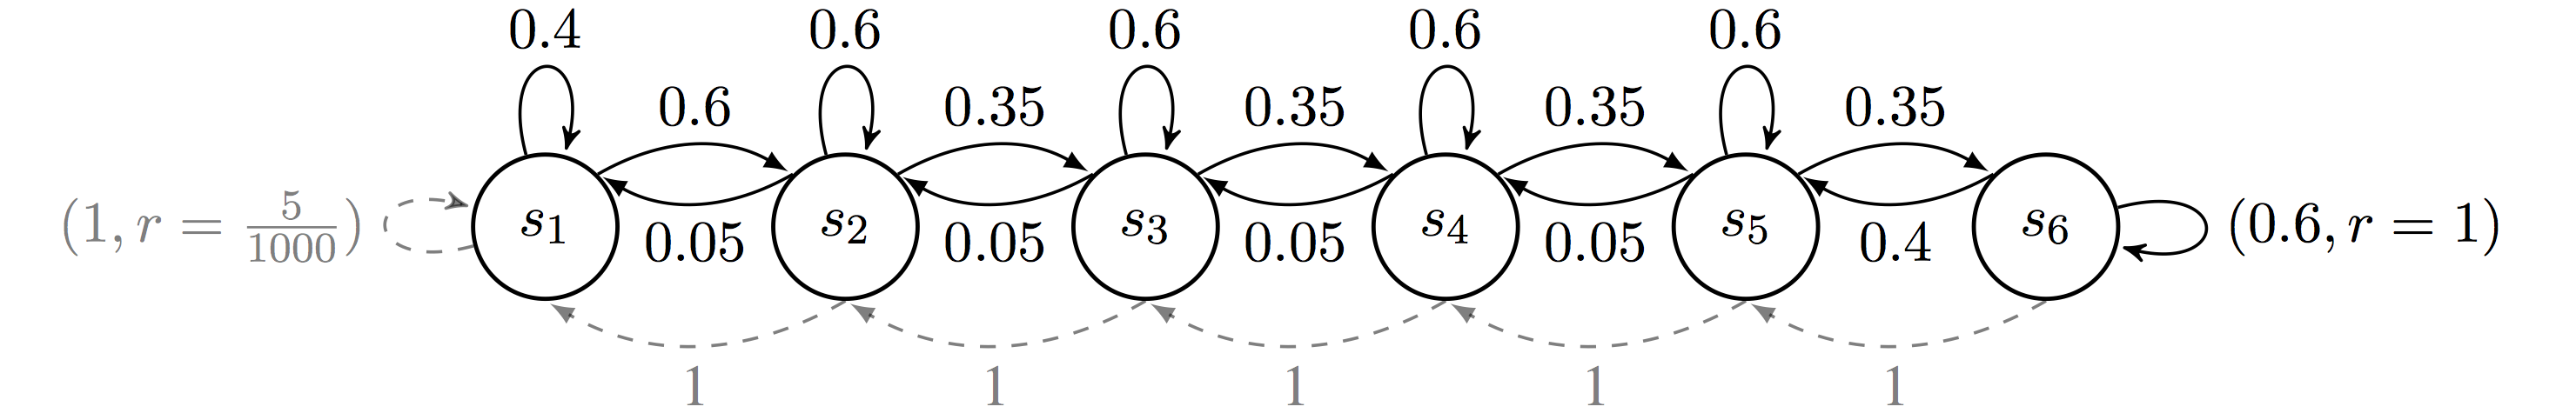
\includegraphics[width=0.9\textwidth]{Diagrams/RiverSwim}      
      \caption{\emph{RiverSwim} - continuous and dotted arrows represent the MDP under the actions ``right" and ``left".}
      \label{figure: RiverSwim}
\end{figure}

\emph{RiverSwim} consists of six states arranged in a chain as shown in Figure \ref{figure: RiverSwim}. The agent begins at the far left state and at every time step has the choice to swim left or right. Swimming left (with the current) is always successful, but swimming right (against the current) often fails. The agent receives a small reward for reaching the leftmost state, but the optimal policy is to attempt to swim right and receive a much larger reward. This MDP is constructed to require efficient exploration to obtain the optimal policy. For the random MDPs we sampled 10-state, 5-action environments according to the prior.

We express our prior in terms of Dirichlet and normal-gamma distributions over the transitions and rewards respectively.\footnote{These priors are conjugate to the multinomial and normal distribution, facilitating efficient posterior updating and sampling. We used the values $ \alpha=1/S , \mu=\sigma^2=1$ and pseudocount $n=1$ for a diffuse uniform prior.}
In both environments we perform 20 Monte Carlo simulations and compute the total regret over 10,000 time steps. We implement UCRL2 with $\delta =0.05$ and optimize the algorithm to take account of finite episodes where appropriate. PSRL outperformed UCRL2 across every environment, as shown in Table 1. In figure \ref{fig:RiverSwim}, we show regret through time across 50 Monte Carlo simulations to 100,000 timesteps in the \emph{RiverSwim} environment, PSRL's outperformance is quite extreme.

%\begin{table}[h!]
%\begin{center}
%\begin{tabular}{| c | c c | c c | }
%\hline
%				& Random MDP	& Random MDP	& \emph{RiverSwim} 	& \emph{RiverSwim} \\
%	Algorithm		& $\tau$ episodes	& $\infty$-horizon 	& $\tau$ episodes	& $\infty$-horizon 	\\
%\hline
%	PSRL		& $1.95 \times 10^5$& $2.25 \times 10^6$&$1.20 \times 10^2$	& $3.30 \times 10^2$ \\
%	UCRL2		&$8.07 \times 10^4$	& $1.26 \times 10^6$&$1.05 \times 10^0$	& $1.49 \times 10^0$ \\
%\hline
%\end{tabular}
%\end{center}
%\caption{Average rewards in simulation. PSRL outperforms UCRL2 across different environments.}
%\label{table:AveRewards}
%\end{table}

\begin{table}[h!]
\begin{center}
\caption{Total regret in simulation. PSRL outperforms UCRL2 across different environments.}
\begin{tabular}{| c | c c | c c | }
\hline
				& \emph{Random MDP}	& \emph{Random MDP}	& \emph{RiverSwim} & \emph{RiverSwim} \\
\emph{Algorithm}		& $\tau$\emph{-episodes}	& $\infty$\emph{-horizo}n 	& $\tau$\emph{-episodes}	& $\infty$\emph{-horizon} 	\\
\hline
	PSRL		& $1.04 \times 10^4$& $7.30 \times 10^3$&$6.88 \times 10^1$	& $1.06 \times 10^2$ \\
	UCRL2		&$5.92 \times 10^4$	& $1.13 \times 10^5$&$1.26 \times 10^3$	& $3.64 \times 10^3$ \\
\hline
\end{tabular}
\end{center}
\label{table: AveRewards}
\end{table}

\subsection{Learning in MDPs without episodic resets}
The majority of practical problems in reinforcement learning can be mapped to repeated episodic interactions for some length $\tau$. Even in cases where there is no actual reset of episodes, one can show that PSRL's regret is bounded against all policies which work over horizon $\tau$ or less\cite{brafman2003r}. Choosing $\tau$ large enough from prior knowledge, we can compete with the optimal policy for any given problem. Alternatively, any setting with discount factor $\alpha$ can be learned to arbitrary accuracy for $\tau \propto (1-\alpha)^{-1}$.

\begin{figure}[h!]
\centering
\begin{subfigure}{.5\textwidth}
  \centering
  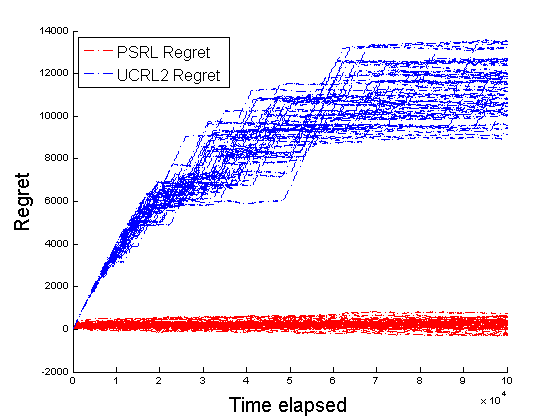
\includegraphics[width=1\linewidth]{Diagrams/combinedGraph.png}
  \caption{PSRL outperforms UCRL2 by large margins}
  \label{fig:sub1}
\end{subfigure}%
\begin{subfigure}{.5\textwidth}
  \centering
  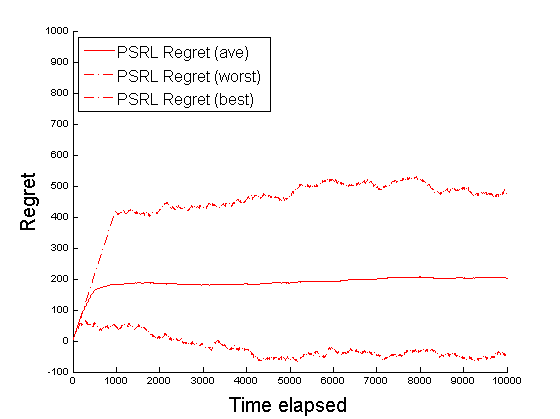
\includegraphics[width=1\linewidth]{Diagrams/psrlGraphShort.png}
  \caption{PSRL learns quickly even with a misspecified prior}
  \label{fig:sub2}
\end{subfigure}
\caption{Simulated regret on the $\infty$-horizon \emph{RiverSwim} environment.}
\label{fig:RiverSwim}
\end{figure}

Nevertheless, for infinite-horizon and undiscounted problems artificially imposing a $\tau$ too small risks overlooking an optimal policy operating over a larger timeframe, whereas a $\tau$ too large may learn slowly. One particularly appealing feature of UCRL2 \cite{jaksch2010near} and REGAL \cite{bartlett2009regal}  is that they learn an optimal timeframe from experience, and replace the factor $\tau$ in \eqref{eq: high probability regret bound} by the diameter and span of the underlying MDP respectively. They both accomplish this by allowing the length of their episodes of fixed policy to vary depending upon the states and actions visited. A new episode is begun, and a policy computed, only when the total visits to any state-action pair is doubled, as opposed to fixed $\tau$-length intervals.

We can apply this same rule for episodes to PSRL, allowing the algorithm to learn more quickly initially, while eventually exploring policies over arbitrarily large timeframes. As shown in figure \ref{fig:RiverSwim} this implementation performs far better than UCRL2, even with a grossly misspecified prior. We see that, while UCRL2's regret grows with the worst case $T$-dependence of $\sqrt{T}$, PSRL performs much better than these bounds and settles upon the optimal policy after only 500 time steps on average.

At present, our analysis for deterministic $\tau$ episodes does not follow through to this infinite horizon extension, since the length episodes of fixed policy is no longer independent observations $H_{t_k}$. For this reason, we are unable to state an equivalent result to (\ref{eq: from Delta to Delta tilde}) relating optimal rewards to those observed by the agent. However, where the optimal average reward of the sampled MDP $M_k$ is uncorrelated with episode length, we can derive results analogous to \cite{jaksch2010near,bartlett2009regal}: that expected regret is $\tilde{O}(S \sqrt{AT \Exp[\Psi^2]})$ where $\Psi$ is the span of bias vector of the optimal MDP $M^*$.




\section{Conclusion}

We establish \emph{posterior sampling for reinforcement learning} not just as a heuristic, but as a provably efficient learning algorithm. We present regret bounds of  $\tilde{O}(\tau S \sqrt{AT} )$, which are some of the first for an algorithm not motivated by optimism and close to state of the art for any reinforcement learning algorithm. These bounds hold in expectation irrespective of prior, and with high probability unless the prior misspecification is exponentially large. PSRL is conceptually simple, computationally efficient and can easily incorporate prior knowledge; we demonstrate that PSRL performs well in simulation. Unusually for algorithms with guaranteed finite-time regret bounds, we have separated our \emph{algorithm} from our \emph{analysis}; as such, it may be possible for further analysis to provide even stronger guarantees on regret. We believe there is a strong case for the wider adoption of algorithms based upon posterior sampling in both theory and practice. 

Looking forward, we are interested in extending our analysis from the episodic case to infinite horizon learning without episodic reset, perhaps through exponentially growing episodes of posterior sampling. We also wonder whether it is possible to match the theoretical lower bounds for regret dependence on the states actions and time elapsed of $\sqrt{SAT}$ \cite{jaksch2010near} through a posterior sampling algorithm. Finally, since most problems of practical interest occur within extremely large, or even infinite, state and action spaces, we would like to explore variants of PSRL which can exploit some simplifying problem structure in these large spaces, such as linearity or factored MDPs.


\newpage

\small{
\bibliography{referenceInformation}
\bibliographystyle{unsrt}
}

\newpage
\appendix
\section{Bounding $\min \left\{\sum_{k\in K_G} \sum_{i=1}^{\tau} \min\left\{ \beta_k^{\delta_2}(s,a), \tau\right\}, \,\, T \right\}$} 

Using the definition of $\beta_k^{\delta_2}(s,a) := \sqrt{\frac{14 S \log(2SAm t_k / \delta_{2})}{\max \{1,N_{t_k}(s,a) \}} }$
we proceed to bound \eqref{eq: final sum} in a manner similar to \cite{jaksch2010near}:
$$ \min \left\{\sum_{k\in K_G} \sum_{i=1}^{\tau} \min\left\{ 2\tau\sqrt{\frac{14 S \log(2SAm t_k / \delta_2)}{\max \{1,N_{t_k}(s,a) \}} }, \tau\right\}, \,\, T \right\}= O\left(\tau S \sqrt{ AT \log(SAT/ \delta_{2})}\right).$$

We split the sum into two parts as: 
\begin{eqnarray}	
\sum_{k\in K_G} \sum_{i=1}^{\tau} \min\left\{ 2\tau\sqrt{\frac{14 S \log(2SAm t_k / \delta_2)}{\max \{1,N_{t_k}(s,a) \}} }, \tau\right\} &\leq& \tau \sum_{k\in K_G}\sum_{i=1}^{\tau}\left[ \mathbf{1}(N_{t_k}(s,a) \leq \tau) \right] \\
&+& 2\tau \sum_{k\in K_G}\sum_{i=1}^{\tau}\left[ \mathbf{1}(N_{t_k}(s,a) > \tau)\sqrt{\frac{14 S \log(2SAT^2 / \delta_2)}{\max \{1,N_{t_k}(s_t,a_t) \}} }  \right] 
\end{eqnarray}

Now, the consider the event $(s_t, a_t)=(s,a)$ and $(N_{t_k}(s,a) \leq \tau)$. This can happen fewer than $2\tau$ times per state action pair. Therefore, $\tau \sum_{k\in K_G}\sum_{i=1}^{\tau}\mathbf{1}(N_{t_k}(s,a) \leq \tau) \leq 2\tau^2 SA$ 

Now, suppose $N_{t_k}(s,a)>\tau$. Then for any $t\in \{t_k,..,t_{k+1}-1\}$, $N_{t}(s,a)+1 \leq N_{t_k}(s,a)+\tau \leq 2N_{t_k}(s,a)$. Therefore 
\begin{equation}
 \sum_{k=1}^{m} \sum_{t=t_k}^{t_{k+1}-1} \sqrt{\frac{\mathbf{1}(N_{t_k}(s_t, a_t)>\tau)}{N_{t_k}(s_t,a_t)}} \leq \sum_{k=1}^{m} \sum_{t=t_k}^{t_{k+1}-1}  \sqrt{\frac{2}{N_{t}(s_t,a_t)+1}} = \sqrt{2} \sum_{t=1}^{T} (N_{t}(s_t, a_t)+1)^{-1/2}
\end{equation}
Now, we can rewrite this sum as: 
$$\sum_{t=1}^{T} (N_{t}(s_t, a_t)+1)^{-1/2} = \sum_{s,a} \sum_{j=1}^{N_{T+1}(s,a)} j^{-1/2} \leq \sum_{s,a} \intop_{x=0}^{N_{T+1}(s,a)} x^{-1/2} dx=2\sum_{s,a} \sqrt{N_{T+1}(s,a)}$$
By the Cauchy-Shwartz inequality, $\sum_{s,a} \sqrt{N_{T+1}(s,a)} \leq \sqrt{SA \sum_{s,a} N_{T+1}(s,a)} =\sqrt{SAT}$. Hence, we have shown that there is a numerical constant $c$ such that 
\begin{eqnarray}
\min \left\{\sum_{k\in K_G} \sum_{i=1}^{\tau} \min\left\{ 2\tau\sqrt{\frac{14 S \log(2SAm t_k / \delta_2)}{\max \{1,N_{t_k}(s,a) \}} }, \tau\right\}, \,\, T \right\} &\leq& \min\left\{ 2\tau^2 SA+c\tau\sqrt{SAT \log(SAT^2)}, \,\,T  \right\} \\
&\leq& \min\left\{ 2\tau^2 SA, \,\,T  \right\}+c\tau\sqrt{SAT \log(SAT^2)}\\
&\leq& \sqrt{2\tau^2 SAT}+c\tau\sqrt{SAT \log(SAT^2)}.
\end{eqnarray}

Which completes the proof.

\end{document}
